% -*- root: ../root.tex -*-
\section[Lecture 1]{Measures} % (fold)
\label{sec:lecture_1}
\begin{defn}
\index{Borel \(\sigma\)-algebraen}Borel \(\sigma\)-algebraen \(\B_k\) på \(\R_k\) er \(\sigal\) frembragt på de åbne mængder \(\os_k\)
\end{defn}
% \begin{exercise}
% Afgør om det er er borel mængder
% \begin{enumerate}[label=(\arabic*)]
%   \item \((\R,\B)\) er et målbart rum.
% \[
%   a,b \Rightarrow A\cup B^c\in\B
% \]
% \item Hvis \(B\subseteq\) er en endelig mængde, så gælder at \(B\in\B\)
% \item \(\{x\}\in\B\) for alle \(x\in\R\)
% \item Hvis \(B\subseteq\R\) er en tællig mængde, så gælder det at \(B\in\B\).
% \item Hvis \(B\subseteq\B\) er overtællig mængde med tællig \(B^c\), så \(B\in\B\)
% \end{enumerate}
% \end{exercise}
% \begin{solution}
% Løsning på overstående
% \begin{enumerate}[label=(\arabic*)]
%   \item Sandt: En \(\sigal\) er \important{stabil} over for  \important{endelige} og  \important{tællige} mængdeoperation
%   \item Falsk: \(\B\ne\pow(\R)\) så findes \(B\in \pow(\R)\) så \(B\in\B\). Så \(\R=B\union B^c\). So if \(B\) er overtællig, så er \(B^c\) også overtællig. Derved er findes der et \(B\notin\B\)
%   \item Sandt:\(\{x\}\) er endelig og \(\B\) indeholder alle \important{endelige!mængder}
%   \item \(B\bigcup_{x\in B}\{x\}\), som er tællig, hvis \(B\) er tællig
%   \item Hvis \(B\) er overtællig, \(B^c\) er tællig, så \(B^c\in\B\), så \(B=(B^c)^c\in B\) (\(B\) er stabil under komplimenter), så \(B\in\B\)
% \end{enumerate}
% \end{solution}

\(\B=\sigma(\os)\), dvs, den mindste \(sigal\) der indeholder \(\os\). F.eks.
\begin{itemize}
  \item De endelige mængder
  \item De åbne kasser \(\I^k\)
  \item De åbne kasser med rationelle hjørner
  \item For \(k=1\), intervaller af formen \((-\infty,b_1],\ldots,\times(-\infty,b_i] \)
\end{itemize}
Lad \(\X\) være en mængde og lad \(\es=\sigma(\X)\), så kaldes \((\X,\es)\) et målbart rum.
\begin{defn}
Et mål \(\mu\) på \((\X,\es)\) er en funktion på \(\es\) som opfylder
\begin{itemize}
  \item \(\mu(A_n)\in[0,\infty]\)
  \item \(\mu(\emptyset)=0\)
  \item \(\mu\left(\bigcup_{n=1}^\infty A_n\right)=\sum_{n=1}^\infty \mu(A_n)\)
\end{itemize}
\end{defn}
\begin{exmp}
Arealet på \((b_i-a_1)(b_2-a_2)\)\tabularnewline
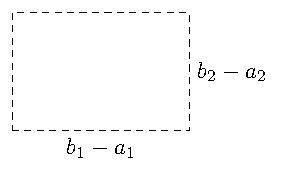
\includegraphics{fig/box.pdf}
\end{exmp}

\subsection{lebesgue målet} % (fold)
\label{sub:lebesgue_m_let}
\begin{defn}
\[
  m_k((a_1,b_1)\times(a_2,b_2)\times\ldots\times(a_k,b_k))=\prod_{i=1}^k(a_i,b_i)
\]
\end{defn}
\subsection{Intergation with respect to a measure} % (fold)
\label{sub:intergation_with_respect_to_a_measure}
When we write something like \(\dif x\) in a integral \(\int f(x) \dif x\) we mean the infinitesimal interval starting at \(x\). So \(\dif x\) tell us 3 things. (i) which variable we are dealing with (ii) the value of that variable, and (iii) the length of a infinitesimal at that value. When we integrate with respect to a measure \(\mu\), we write \(\mu(\dif x)\), which is short hand for \(\mu(x,x+\dif x)\). That is the measure of a infinitesimal change in interval starting at \(x\). So in a intergral
\[
  \int f(x) \mu(\dif x)
\]
\(f(x)\) is the height and \(\mu(\dif x)\) is the lenght of the infinitisimal area \(f(x) \mu(\dif x)\)
% subsection intergation_with_respect_to_a_measure (end)
% \begin{exercise}
% Afgør om følgende er sandt eller falsk
% \begin{enumerate}
%   \item hvis \(A\subseteq B\) med \(\mu(A)=0\) og \(B\subseteq A\) så \(B\in \B\)
%   \item \(\mu(\R)=\lim_{n \rightarrow \infty}\mu[-n,n]\)
%   \item \(\mu(\{0\})=\lim_{n \rightarrow \infty}(\left[-n^{-1},n^{-1}\right])\)
%   \end{enumerate}
% \end{exercise}

% \begin{solution}
% Løsninger på overstående
% \begin{enumerate}
%   \item  Falsk: Der findes (for f.eks. lebesgue målet) ikke målige nul mængder. Dvs. \(B\subseteq A\), hvor \(\mu(A)=0\), og \(B\in\R\)
% \item Sandt: \(\R=\bigcup_{n\in\N}[-n,n]\) og \(\left[-n,n\right]\) vokser opad (dvs. \([-1,1]\subseteq[-2,2]\subseteq\ldots\subseteq [-n,n]\). Da målet er opad kontinuert, så er \(\mu\bigcup_n[-n,n]=\lim_{n \rightarrow \infty}\mu\bigcup_n[-n,n]\)
% \item Falsk: \(\{0\}=\bigcap_{n\in\N}\left[-n^{-1},n^{-1}\right]\). Tag f.eks. tællemålet \(\mu=\tau\). \(\tau(\{0\})=1\) men \\ \(\tau\left[-n^{-1},n^{-1}\right]=\infty\)
% \end{enumerate}
% \end{solution}
